\documentclass[a4paper,12pt]{article}

\RequirePackage{epsfig}

\setlength\hoffset{-0.5in}      %% these work quite well with a 12pt font
\setlength\voffset{-0.5in}
\setlength{\textwidth}{6.30in}
\setlength{\textheight}{9.0in}

\usepackage{graphicx}
\graphicspath{ {./img/} }

\bibliographystyle{unsrt}
\begin{document}

\begin{center}
{\Large\bf{Decentralised Blockchain Security Architecture for IoT and MQTT Brokers}} \\
      \vspace{5.0mm}
{\Large\bf{Project Plan}} \\
      \vspace{8mm}
      {\large\bf{Konrad Dryja}}  \\
      \vspace{5.0mm}
       {\tt k.dryja.15@abdn.ac.uk} \\
      \vspace{5.0mm}
      {\em Department of Computing Science,\\
       University of Aberdeen, Aberdeen AB24 3UE, UK} 
\end{center}


\section*{Introduction}

IoT is a growing field with presence getting larger from day to day. Equipment such as bus timetables, doorbells, thermostats or even pacemakers capable of sending alerts directly to emergency services is omnipresent. Sensitive data is very often handled (especially in the last example) and leak or misrepresentation can have catastrophic consequences. Additionally, those devices have limited computation power, which is sacrificed in favour of extended lifespan to avoid frequent maintenance and/or battery replacement. This makes it a very lucrative target for malicious actors. Researchers from University of Michigan performed a demo attack on a pacemaker, extracting personal information and changing the configuration.\cite{4531149} This example and more clearly presents a need for solution capable of securing and closing off access to unwanted agents.

What is more, those devices frequently do not directly communicate on a peer-to-peer basis, but instead pass through intermediary resource handling the distribution of data. MQTT Brokers\footnote{https://mqtt.org/} are one of them, providing a Publisher/Subscriber architecture, allowing for information exchange without the constant need of interconnectivity between clients, instead of relying on created topics used as a relay. MQTT is also not a piece of software, but rather a standard describing the operation of such backend and leaves the implementation up to end-users. The documentation also clearly states that the security is not a part of the standard, but rather leaves this decision up to the implementors, offering several alternatives\footnote{https://docs.oasis-open.org/mqtt/mqtt/v5.0/os/mqtt-v5.0-os.html\#\_Toc3901261}. And while the transport of data can be assumed to remain secure (as MQTT operates over TCP/IP, thus encrypting the data using TLS), the access is often not. For example, an attack could be conducted, where malicious device communicates with the broker, impersonating another IoT hardware and finally compromise confidentiality, as shown on Figure~\ref{fig:iot1}.

\begin{figure}[ht]
  \centering
  \caption{Attackers can impersonate IoT devices}\label{fig:iot1}
  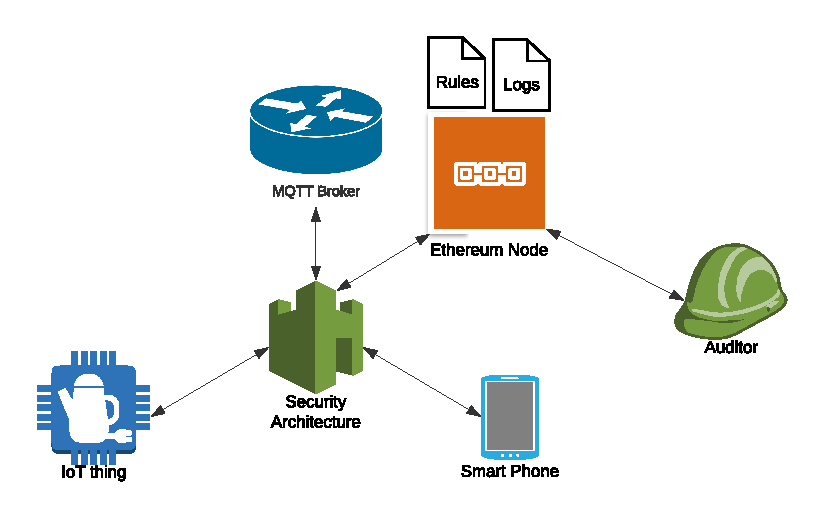
\includegraphics[scale=0.8]{iot_attack}
\end{figure}

Common implementation of MQTT brokers includes basic authentication based on a username and a secret password, offering limited to no logging capabilities. For example, one of the most popular brokers being Mosquitto\footnote{https://mosquitto.org/man/mosquitto-conf-5.html}, as of version 1.6.8 offers password based authentication with ACL capabilities restricting some credentials only to given topics. TrustLens project from University of Aberdeen presented solution of attaching semantic annotations to ongoing operation of a broker and in process allowing higher transparency of broker's state\cite{10.1145/3366610.3368099}.

I would like to propose a universal, pluggable module following the description of MQTT standard (and thus potentially making it independent from the used MQTT implementation) handling Authentication, Authorization and Accountability of IoT devices and consumers attempting connection to the brokers. In order to make the platform more resilient and independent from single points of failure (often being the central ACL repository), I will deploy it on a blockchain - which by convention supports recording of transactions (by recording them on the blockchain) and authentication via ID of the presented wallet. I will also be aiming to merge the efforts of Aberdeen's scientist into the project, enhancing trust of captured data.

Preliminary research revealed similar efforts by scientist in Khon Kaen University~\cite{8523942}, although focusing mostly on Hyperledger Fabric and optimization of the configuration through Genetic Algorithms. The paper doesn't make any mention of logging and provenance functionality, which I would like to put more attention towards - along with focusing on Ethereum platform instead.


\section*{Goals}

The project can be divided onto main goals and extras, leaving some field for maneuvering in case of road blocks or difficulties resulting from the challenges faced in the dissertation. By having flexible targets, I will be able to stop sooner in case of overestimating the schedule, or carrying on with extra work, should I find myself meeting the targets quicker than expected. Moreover, I would like to also put some attention to listing the things that the project is \textbf{not} trying to be, to avoid sidetracking.

\paragraph{Main Goals:}
\begin{itemize}
  \item Design Blockchain network and deploy on Ethereum platform, capable of recording transactions and allowing for modification of ACLs, i.e. which wallet ID is permitted to access given topics.
  \item Design containerised software acting as a secure proxy between brokers and connecting clients.
  \item Deploy and test on at least one MQTT implementation (e.g. Moquette, Mosquitto), simulated with software.
\end{itemize}

\paragraph{Extra Goals:}
\begin{itemize}
  \item Explore and implement implementation of the architecture to any, arbitrary broker.
  \item Connect physical LoRaWAN gateways to the software.
\end{itemize}

\paragraph{No-goals:}
\begin{itemize}
  \item Design a new blockchain platform from scratch.
\end{itemize}


\section*{Methodology}

This section should describe {\em how} you will conduct
your project. You should explain in general terms
the activities you will be carrying out during your project, such as:
%
\begin{itemize}
\item reading about related work -- either to get ideas on how to
      proceed, or to compare your approach with what was done before;
\item learing a new programming language or API;
\item learning about relevant technologies;
\item developing prototypes to test ideas;
\item testing and debugging early design choices.
\end{itemize}
%
The above examples are purely suggestions. You should try to think
of what would be appropriate for your specific project.

\section*{Resources Required}

For the purposes of the project, laptop and a workstation should be sufficient, as the MQTT brokers can be simulated via software, without the need of physical IoT devices sending the messages. For the second stage of the project, I will be considering putting the software on a physical LoRaWAN gateway, enhancing the current broker implementation. TrustLens team from University of Aberdeen recently acquired such gateway, which I will be able to use given the need. Moreover, the team also owns several PuckJS sensors and Arduino boards, which would allow to deploy the whole system and test its behaviour in the real world.

To summarize the requirements:
\begin{itemize}
  \item Linux PC with the following software: 
    \begin{itemize}
      \item Golang 1.12+ 
      \item Docker 19.03.5+
      \item Suitable code editor (Vim)
    \end{itemize}
  \item Additionally, for tests in the field:
    \begin{itemize}
      \item LoRaWAN Gateway
      \item IoT sensors (PuckJS, Arduino) 
    \end{itemize}
\end{itemize}

\section*{Risk Assessment}

Try to describe possible circumstances (e.g. a particular piece of
technology doesn't work or is too expensive) that might cause
the project to become become infeasible. What would you have to do
or change to recover your project?

\section*{Timetable}

This section should describe the {\em schedule} for your project. 
You should describe the various activities you expect to perform
and their durations, along with any deadlines and deliverables.
It is often useful to collect all of this information in a
{\em Gantt chart}, as shown in Figure~\ref{fig:plan} below:

\begin{figure}[htb]
\begin{center}
% \includegraphics[scale=0.65]{ProjectPlan.eps}
\caption{Main Project Activities\label{fig:plan}}
\end{center}
\end{figure}

% For information, this figure was created using xfig, and 
% converted to encapsulated postscript by a command in the Makefile
% before being included as a graphic in the \LaTeX document.

Don't forget to add time at the end of your project for 
evaluation and writing-up! This could easily require 2-3 weeks.


\bibliography{ProjectPlan}

\end{document}
